\documentclass[aspectratio=169,11pt]{beamer}
\usepackage{iftex}
\ifPDFTeX
  \usepackage[utf8]{inputenc}
  \usepackage[T1]{fontenc}
\else
  \usepackage{fontspec}
  \usepackage{xeCJK}
  \setmainfont{Latin Modern Sans}
  \setsansfont{Latin Modern Sans}
  \setCJKmainfont{FandolSong-Regular}
\fi
\usepackage{graphicx}
\usepackage{booktabs}
\usepackage{array}
\usepackage{tabularx}
\usepackage{hyperref}

\usetheme{Madrid}
\usecolortheme{default}
\definecolor{PrimaryBlue}{RGB}{17,82,147}
\definecolor{AccentBlue}{RGB}{45,117,191}
\definecolor{SoftBlue}{RGB}{233,241,250}
\setbeamercolor{structure}{fg=PrimaryBlue}
\setbeamercolor{title}{fg=white,bg=PrimaryBlue}
\setbeamercolor{frametitle}{fg=white,bg=PrimaryBlue}
\setbeamercolor{block title}{fg=white,bg=PrimaryBlue}
\setbeamercolor{block body}{fg=black,bg=blue!4}
\setbeamercolor{itemize item}{fg=AccentBlue}
\setbeamerfont{title}{series=\bfseries,size=\Large}
\setbeamerfont{frametitle}{series=\bfseries,size=\large}
\setbeamertemplate{navigation symbols}{}
\setbeamertemplate{headline}{}
\setbeamertemplate{footline}[frame number]

\title[Midterm]{Red-Teaming Large Language Model-Powered\\Recommendation Systems}
\subtitle{Midterm Presentation: RAG Poison Lab Framework, Attack Workflow, and Experiment Pipeline}
\author[Sbaaoui Idriss]{Sbaaoui Idriss\\Student ID: 22060004}
\institute[ECUST]{Computer Science, 华东理工大学\\Supervisor: 张恒润}
\date{April 2026}

\begin{document}

\begin{frame}[plain]
  \titlepage
\end{frame}

\begin{frame}{Why this project exists}
\begin{itemize}
  \item Modern recommendation systems increasingly combine retrieval, ranking, and LLM-based reasoning in one pipeline.
  \item If indexed content is poisoned, the final recommendation output can change without retraining the model.
  \item \textbf{RAGPoison} exists as a controllable local lab to trace that effect from data preparation to final top-$K$ output.
  \item The project goal is practical: measure how poisoning changes retrieval evidence, ranking, and user-visible recommendations.
\end{itemize}
\end{frame}

\begin{frame}{RAG Poison Lab framework overview}
\begin{columns}[T,totalwidth=\textwidth]
\column{0.50\textwidth}
\begin{block}{Core workflow}
\begin{enumerate}
  \item Prepare MovieLens 100K data
  \item Export baseline bulk and poisoned bulk
  \item Index \texttt{movies} and \texttt{movies\_poisoned}
  \item Run baseline vs attacked evaluation
  \item Save metrics, traces, and reports
\end{enumerate}
\end{block}

\column{0.46\textwidth}
\begin{block}{Main subsystems}
\begin{itemize}
  \item FastAPI backend
  \item Poisoning/attack builder
  \item Elasticsearch retrieval layer
  \item Evaluation and reporting
  \item React demo frontend
\end{itemize}
\end{block}
\vspace{0.4em}
{\footnotesize Evidence: \texttt{README.md}, \texttt{api/app/}, \texttt{agent/}, \texttt{rag/}, \texttt{web/src/}}
\end{columns}
\end{frame}

\begin{frame}{Architecture and tools}
  \centering
  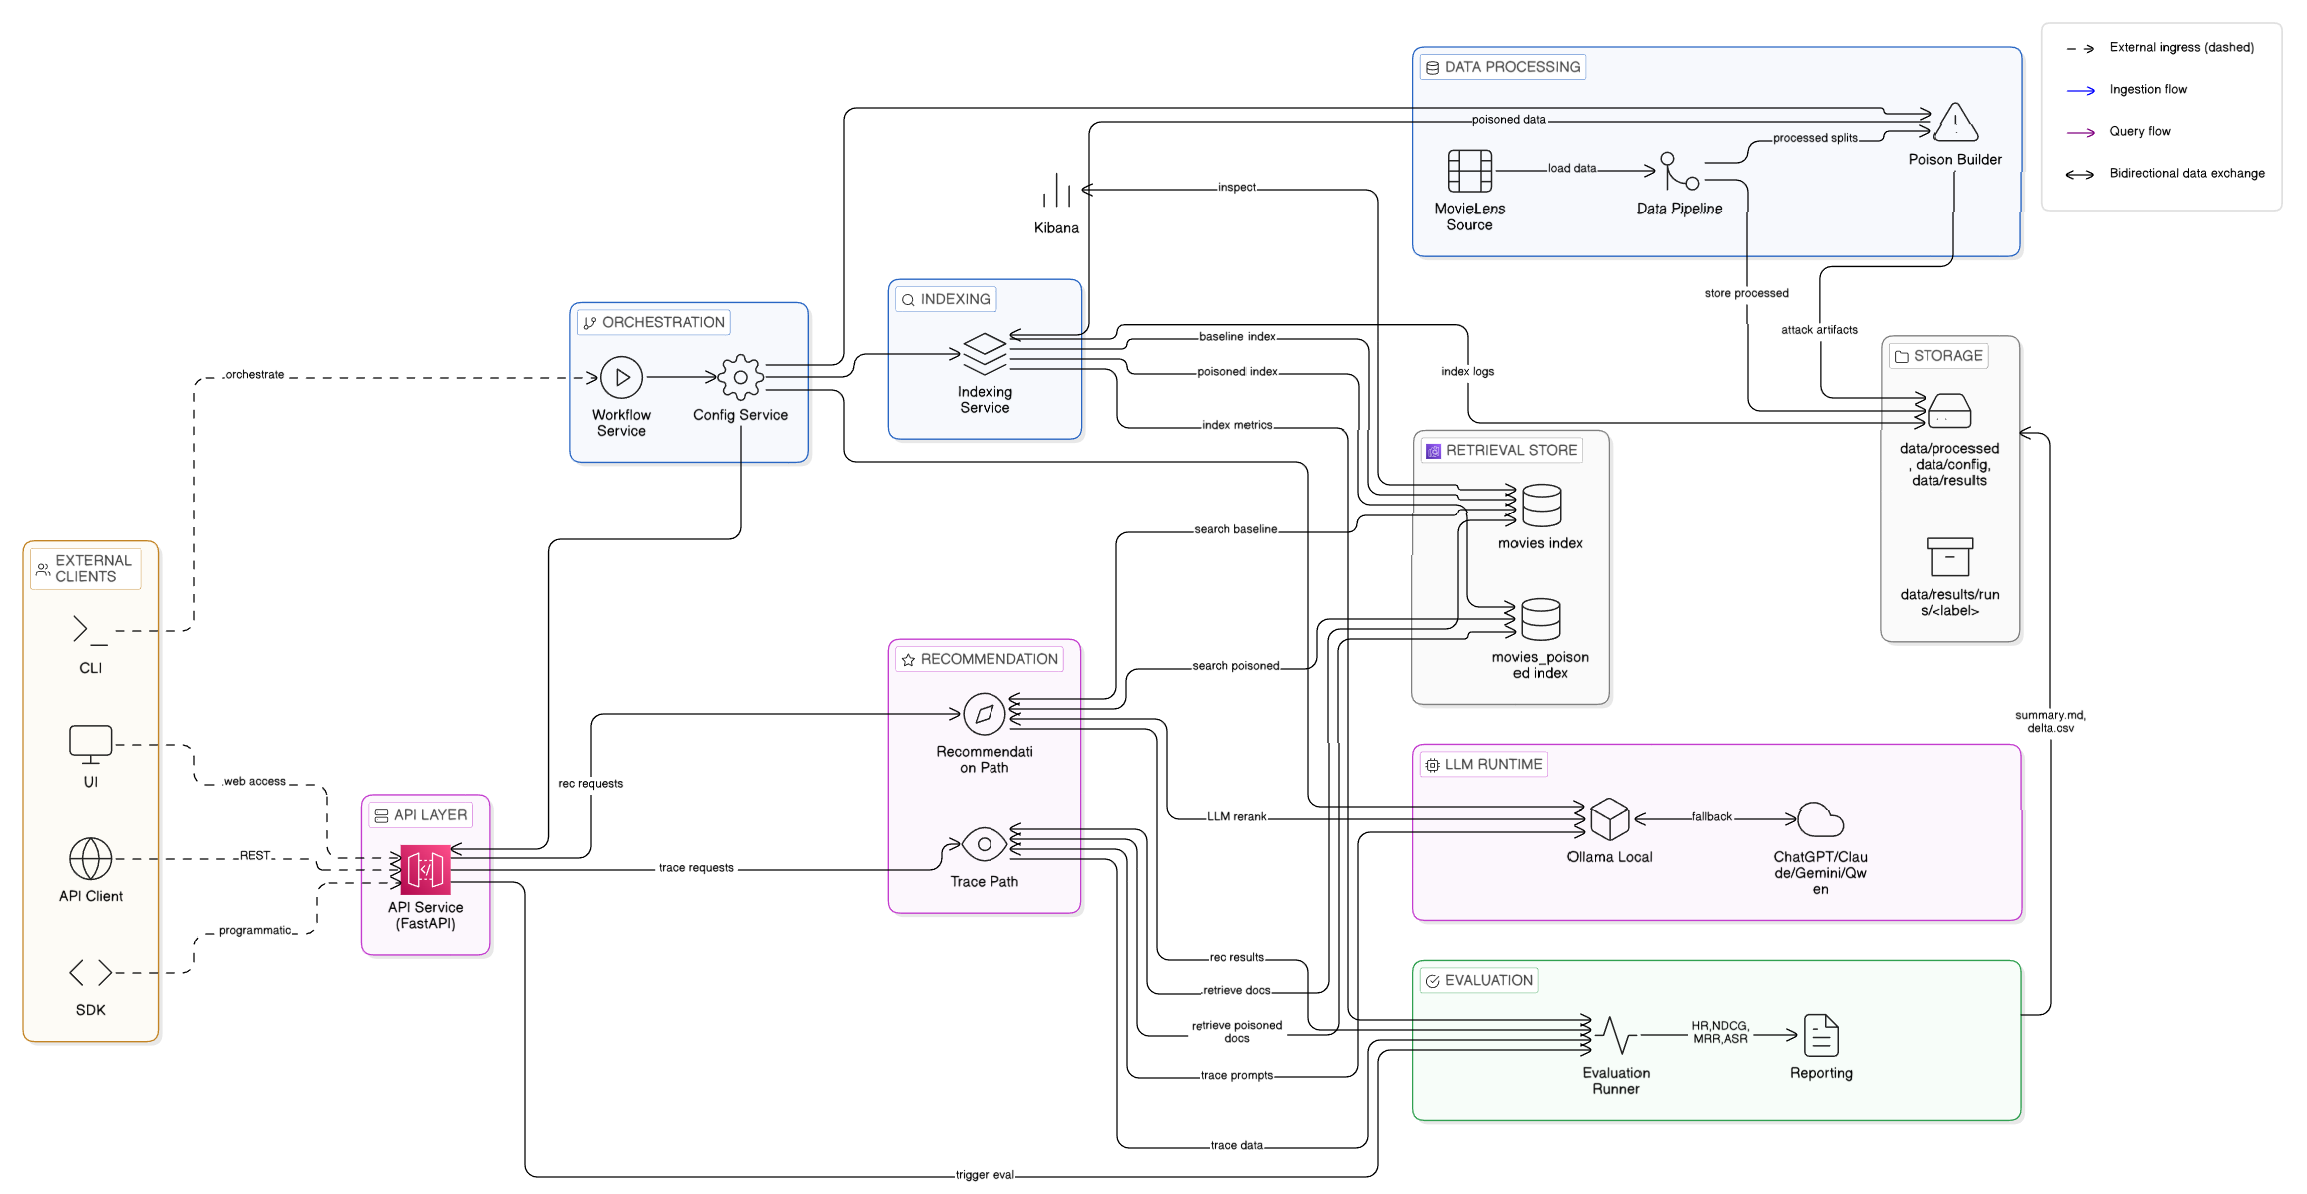
\includegraphics[width=0.95\textwidth]{figures/architecture.png}
\vspace{0.3em}

{\footnotesize
Tooling in the current repo: FastAPI, React/Vite, Elasticsearch, Kibana, Docker Compose, \texttt{uv}, local/cloud LLM providers, and a Python SDK.}
\end{frame}

\begin{frame}{Dataset and indexing pipeline}
\begin{columns}[T,totalwidth=\textwidth]
\column{0.58\textwidth}
\begin{itemize}
  \item Dataset: MovieLens 100K loaded into movies, ratings, temporal splits, and user profiles.
  \item Preprocess stage writes \texttt{movies.parquet}, \texttt{ratings.parquet}, \texttt{splits.parquet}, and \texttt{user\_profiles.parquet}.
  \item Elasticsearch bulk export produces clean \texttt{es\_bulk\_movies.jsonl} and poison-ready \texttt{es\_bulk\_poisoned\_movies.jsonl}.
  \item Indexing resolves mappings, validates bulk payloads, creates versioned physical indices, and swaps aliases.
\end{itemize}

\column{0.38\textwidth}
\begin{block}{Index surfaces}
\begin{itemize}
  \item \texttt{movies}
  \item \texttt{movies\_poisoned}
  \item BM25 lexical mapping
  \item dense / hybrid retrieval support
\end{itemize}
\end{block}
\end{columns}
\end{frame}

\begin{frame}{Clean vs poisoned recommendation workflow}
  \centering
  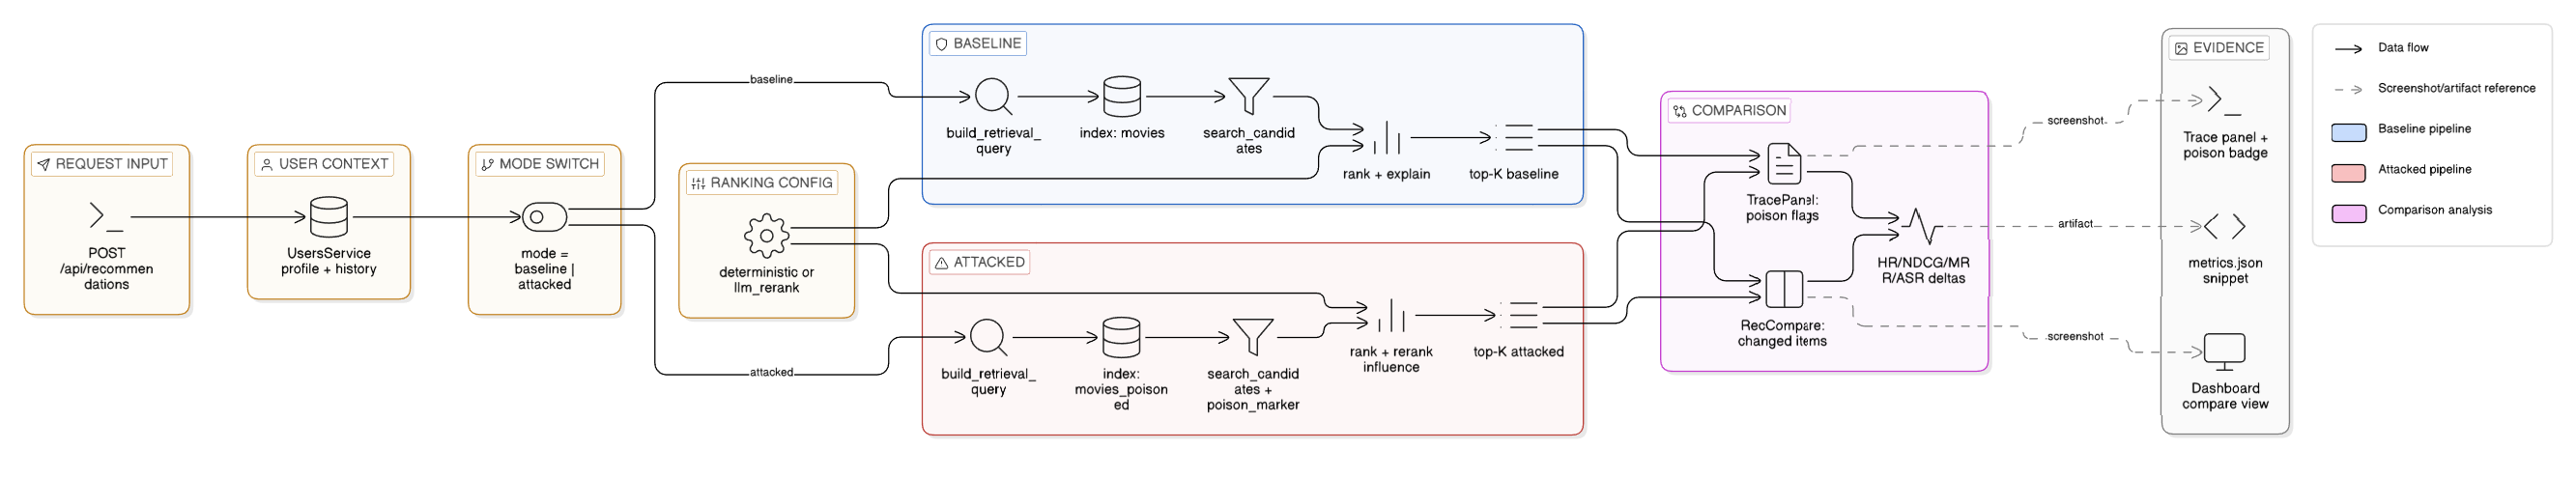
\includegraphics[width=0.98\textwidth]{figures/baseline_vs_attacked_workflow.png}
\vspace{0.2em}

{\footnotesize Same user context and top-$K$ target, different retrieval corpus: baseline index vs poisoned index.}
\end{frame}

\begin{frame}{Attack types and experiment workflow}
\begin{columns}[T,totalwidth=\textwidth]
\column{0.48\textwidth}
\begin{block}{Implemented / configured attacks}
\begin{itemize}
  \item \textbf{targeted\_promotion}
  \item \textbf{prompt\_injection}
  \item \textbf{untargeted\_degradation}
\end{itemize}
\end{block}
\begin{block}{Attack controls}
\begin{itemize}
  \item poison fraction
  \item target movie id
  \item payload text
  \item keyword burst / aggressive boost
  \item target fields: title, genres, synopsis
\end{itemize}
\end{block}

\column{0.48\textwidth}
\begin{block}{Experiment execution}
\begin{enumerate}
  \item set \texttt{attack\_config.json}
  \item prepare data
  \item build poisoned bulk
  \item index baseline + attacked corpora
  \item run single / batch / full eval
  \item generate \texttt{metrics.json}, \texttt{attack\_trace.json}, \texttt{summary.md}
\end{enumerate}
\end{block}
\end{columns}
\end{frame}

\begin{frame}{Metrics and evaluation logic}
\small
\begin{tabularx}{\textwidth}{>{\raggedright\arraybackslash}p{0.24\textwidth} >{\raggedright\arraybackslash}X}
\toprule
Metric / evidence & What it measures in this project \\
\midrule
HR@K & whether at least one relevant movie appears in the final top-$K$ \\
NDCG@K & recommendation quality with position-aware gain \\
MRR@K & first-hit quality in the ranked list \\
ASR@K & whether the configured target movie appears in the final top-$K$ \\
Target retrieval rank / presence & whether the target enters retrieval and how far it moves before final ranking \\
Trace + fallback metadata & whether reranking, strict retrieval, or fallback behavior affected interpretation \\
Latency & not yet a standard exported run metric in the current artifact set \\
\bottomrule
\end{tabularx}
\vspace{0.4em}

{\footnotesize Metrics are implemented in \texttt{api/app/eval/metrics.py}; per-run evidence is saved in \texttt{metrics.json}, \texttt{attack\_trace.json}, and report artifacts.}
\end{frame}

\begin{frame}{Frontend demo role and live walkthrough}
\begin{columns}[T,totalwidth=\textwidth]
\column{0.49\textwidth}
\begin{block}{What the frontend is for}
\begin{itemize}
  \item inspect settings and attack configuration
  \item run experiments from the web UI
  \item stream live orchestration logs
  \item compare run outputs in a presentation-friendly view
  \item inspect traces and recommendation diffs
\end{itemize}
\end{block}

\column{0.47\textwidth}
\begin{block}{Tonight's demo flow}
\begin{enumerate}
  \item show Settings / attack configuration
  \item launch a single-user experiment
  \item follow SSE log stream in Experiments
  \item open Results and the run summary
  \item inspect trace / recommendation comparison
\end{enumerate}
\end{block}
\vspace{0.3em}
{\footnotesize Current recommended live path: deterministic ranking + lexical retrieval + targeted promotion demo config.}
\end{columns}
\end{frame}

\begin{frame}{Current status, remaining work, and results placeholder}
\begin{columns}[T,totalwidth=\textwidth]
\column{0.49\textwidth}
\begin{block}{Current implementation status}
\begin{itemize}
  \item data preparation pipeline implemented
  \item poisoning and index build workflow implemented
  \item baseline / attacked evaluation implemented
  \item metrics, traces, and reports implemented
  \item frontend demo surfaces implemented
\end{itemize}
\end{block}

\column{0.47\textwidth}
\begin{block}{What remains}
\begin{itemize}
  \item finalize experiment matrix and thesis-grade analysis
  \item stabilize provider-dependent rerank demos
  \item decide final result tables/figures for the thesis
  \item add finalized conclusion only after experiment lock
\end{itemize}
\end{block}
\end{columns}
\end{document}
